\section{Existing Tools}

\begin{frame}
	\frametitle{Minimap}
	\begin{itemize}
		\item<1-> Used Minimizer and Min-sketch
		\item<1-> Tweaked for Miniasm
		\item<1-> Multi-threaded
		\item<1-> Not Tested Enough Yet
	\end{itemize}
	\begin{alertblock}{Output Format}
		The output format is PFA which is different than other tools.
	\end{alertblock}
\end{frame}

\begin{frame}
	\frametitle{BWA}
	\begin{itemize}
		\item<1-> Two versions:
			\begin{itemize}
				\item<1-> BWA / BWA-MEM for Illumina/Solexa reads
				\item<1-> BWA-SW for Oxford Nanopore Reads of MinION instrument
			\end{itemize}			
		\item<1-> Used BWT
		\item<1-> Used Prefix-Trie Traversing Top-Down Fashion
		\item<1-> Applied Smith–Waterman-like Dynamic Programming
		\item<1-> Multi-threaded
	\end{itemize}
\end{frame}

%Gaurab vai
\begin{frame}
	\frametitle{Bowtie}
	\begin{itemize}
		\item<1-> Two versions:
		\begin{itemize}
			\item<1-> Bowtie 
			\item<1-> Bowtie 2
		\end{itemize}			
		\item<1-> Used BWT FM-index
		\item<1-> Quality-aware Backtracking Algorithms Enabling Mismatches
		\item<1-> Double Indexing  -- To Avoid the Excessive Use of Backtracking
	\end{itemize}
\end{frame}

%Gaurab vai
\begin{frame}
	\frametitle{MUMmer}
	\begin{itemize}
		\item<1-> Three versions: 1, 2, 3			
		\item<1-> Used Suffix-Tree
	\end{itemize}
\end{frame}

\begin{frame}
	\frametitle{NanoBLASTer}
	\begin{itemize}
		\item<1-> Used "seed-and-extend" Technique
		\item<1-> Dynamic Programming Based	Extension Mechanism
		\item<1-> Faster than Leading Alignment Tools
		\item<1-> Less False Positive Rate
		\begin{alertblock}{Limitation}
			Could not Handle Long Insertion or Deletion
		\end{alertblock}
	\end{itemize}
\end{frame}

\begin{frame}
	\frametitle{Long Insertion}
	\begin{figure}
		\centering
		
		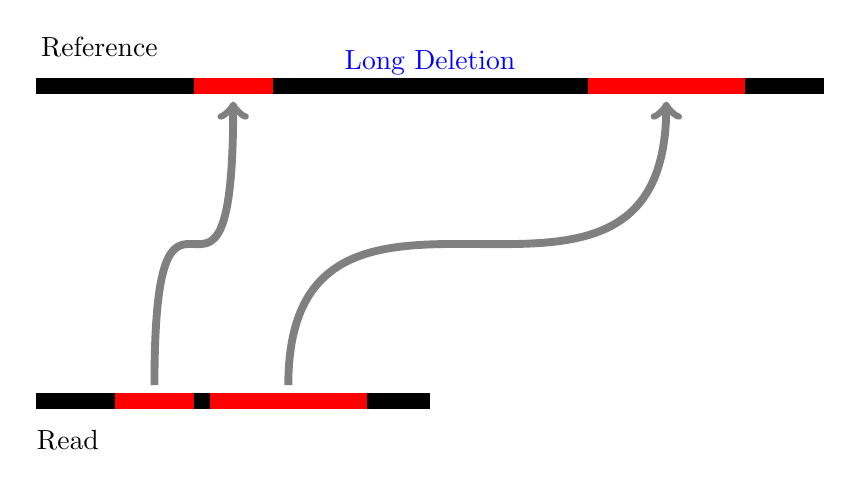
\begin{tikzpicture}[]
		
		%reference
		\draw[line width=2mm] (0,4) -- (10,4);
		\draw[line width=2mm,color=red] (2,4) -- (3,4);
		\draw[line width=2mm,color=red] (7,4) -- (9,4);
		%read
		\draw[line width=2mm] (0,0) -- (5,0);
		\draw[line width=2mm,color=red] (1,0) -- (2,0);
		\draw[line width=2mm,color=red] (2.2,0) -- (4.2,0);
		%labels
		\node[rectangle](refer) at (0.8,4.5) {Reference};
		\node[rectangle,color=blue](refer) at (5,4.3) {Long Deletion};
		\node[rectangle](refer) at (0.4,-0.5) {Read};
		%arrows
		\draw[line width=1mm,color=black!50,->] (1.5,0.2) ..  controls (1.5,3.8) and (2.5,0.2) .. (2.5,3.8);
		\draw[line width=1mm,color=black!50,->] (3.2,0.2) .. controls(3.2,3.8) and (8,0.2) .. (8,3.8);
		\end{tikzpicture}
		\caption{Mapping Two Long K-mers with Long Deletion in Read.}
		\end{figure}
		
\end{frame}

\begin{frame}
	\frametitle{Long Deletion}
	\begin{figure}
		\centering
		
		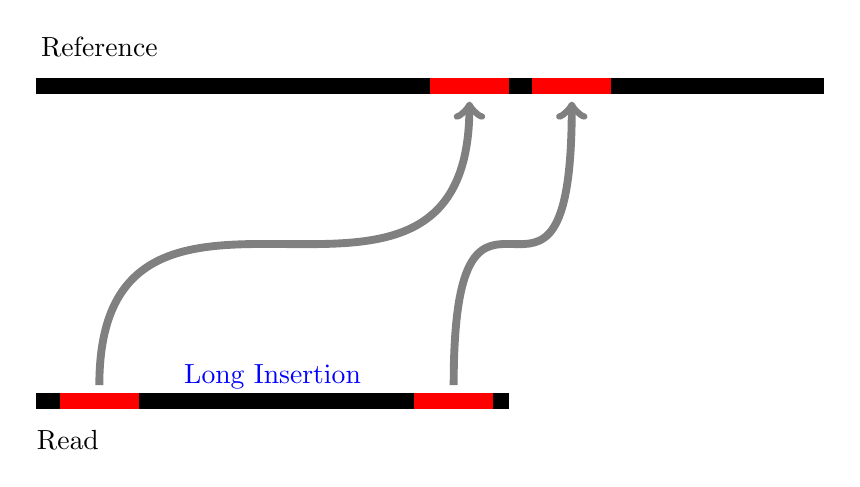
\begin{tikzpicture}[]
		%reference
		\draw[line width=2mm] (0,4) -- (10,4);
		\draw[line width=2mm,color=red] (5,4) -- (6,4);
		\draw[line width=2mm,color=red] (6.3,4) -- (7.3,4);
		%reads
		\draw[line width=2mm] (0,0) -- (6,0);
		\draw[line width=2mm,color=red] (0.3,0) -- (1.3,0);
		\draw[line width=2mm,color=red] (4.8,0) -- (5.8,0);
		%labels
		\node[rectangle](refer) at (0.8,4.5) {Reference};
		\node[rectangle,color=blue](refer) at (3,0.3) {Long Insertion};
		\node[rectangle](refer) at (0.4,-0.5) {Read};
		%arrows
		\draw[line width=1mm,color=black!50,->] (0.8,0.2) ..  controls (0.8,3.8) and (5.5,0.2) .. (5.5,3.8);
		\draw[line width=1mm,color=black!50,->] (5.3,0.2) .. controls(5.3,3.8) and (6.8,0.2) .. (6.8,3.8);
		\end{tikzpicture}
		\caption{Mapping Two Long K-mer with Long Insertion in Read.}
		\end{figure}
\end{frame}